% Chapter 3

\chapter{SCATS Volume Data} % Main chapter title

% For referencing the chapter elsewhere, use \ref{Chapter3}
\label{Chapter3}

% This is for the header on each page - perhaps a shortened title
\lhead{Chapter 3. \emph{SCATS Volume Data}}

%----------------------------------------------------------------------------------------
% Quotation
``There is no order in the world around us, we must adapt ourselves to the requirements of chaos
instead."

\begin{flushright}
Kurt Vonnegut, \textit{Breakfast of Champions} (1973)
\end{flushright}

%---------------------------------------------------------------------------------------------------
%	CONTENT
%   Reference - http://www.scats.com.au/files/an_introduction_to_scats_6.pdf
%---------------------------------------------------------------------------------------------------
\section{Introduction}
SCATS(Sydney Coordinated Adaptive Traffic System) is an adaptive traffic control system. It was
developed by the Department of Main Roads in the 1970's. SCATS operates in real-time by adjusting
signal timings in response to changes in traffic demand and road capacity. All major and minor
cities in Australia and New Zealand use SCATS. Few other cities around the world such as Hong
Kong, Kuala Lumpur, Sanghai and Singapore also have adopted SCATS over other adaptive traffic
control system. In Melbourne and surrounding cities, SCATS controls more than 3,900 sets of traffic
signals

There are three main parameters that SCATS user to achieve traffic signal coordination:
\begin{itemize}
\item[\tiny{$\blacksquare$}] Cycle time: The total time of all signal sequences in a cycle
\item[\tiny{$\blacksquare$}] Phase split: The proportion of the cycle time allocated to each phase
\item[\tiny{$\blacksquare$}] Offset: The time relationship between the starting and finishing of
the green phases of succesive sets of signals within a coordinated system
\end{itemize}

The desicion making of the SCATS system occurs at two levels - \emph{strategic} and \emph{tactical}.


\section{Volume data}
Traffic loop detectors are embedded in the raod pavement and located in each lane near the stop
line at traffic intersections. These detectors collect traffic volume and the time it takes a
vehicle to clear the loop.


\subsection{Handling missing data}


\section{Exploratory analysis}
Figure \ref{fig:AverageTrafficVolume} shows the daily, weekly, monthly and yearly average traffic
volume at a site
location.

\begin{figure}[htbp]
  \centering
    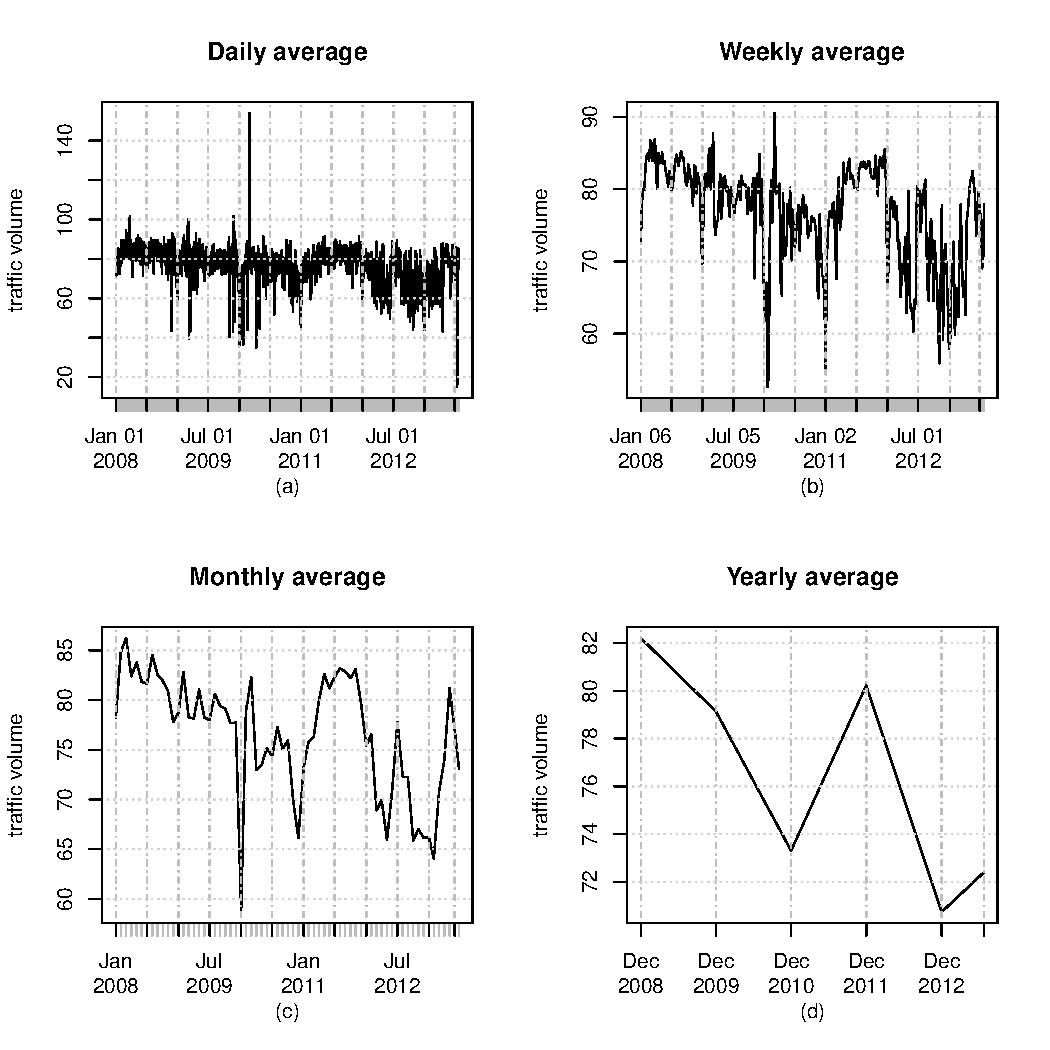
\includegraphics[width=\textwidth,height=\textheight,keepaspectratio]{Figures/averages.pdf}
    \rule{35em}{0.5pt}
  \caption[Average Traffic Volume]{(a) daily, (b) weekly, (c) monthly and (d) yearly average of
  traffic volume (15 mins interval) at a site location from the period 01/01/2008 to 26/07/2013}
  \label{fig:AverageTrafficVolume}
\end{figure}
